\documentclass[twoside]{book}

% Packages required by doxygen
\usepackage{fixltx2e}
\usepackage{calc}
\usepackage{doxygen}
\usepackage[export]{adjustbox} % also loads graphicx
\usepackage{graphicx}
\usepackage[utf8]{inputenc}
\usepackage{makeidx}
\usepackage{multicol}
\usepackage{multirow}
\PassOptionsToPackage{warn}{textcomp}
\usepackage{textcomp}
\usepackage[nointegrals]{wasysym}
\usepackage[table]{xcolor}

% NLS support packages
\usepackage[T2A]{fontenc}
\usepackage[russian]{babel}

% Font selection
\usepackage[T1]{fontenc}
\usepackage[scaled=.90]{helvet}
\usepackage{courier}
\usepackage{amssymb}
\usepackage{sectsty}
\renewcommand{\familydefault}{\sfdefault}
\allsectionsfont{%
  \fontseries{bc}\selectfont%
  \color{darkgray}%
}
\renewcommand{\DoxyLabelFont}{%
  \fontseries{bc}\selectfont%
  \color{darkgray}%
}
\newcommand{\+}{\discretionary{\mbox{\scriptsize$\hookleftarrow$}}{}{}}

% Page & text layout
\usepackage{geometry}
\geometry{%
  a4paper,%
  top=2.5cm,%
  bottom=2.5cm,%
  left=2.5cm,%
  right=2.5cm%
}
\tolerance=750
\hfuzz=15pt
\hbadness=750
\setlength{\emergencystretch}{15pt}
\setlength{\parindent}{0cm}
\setlength{\parskip}{3ex plus 2ex minus 2ex}
\makeatletter
\renewcommand{\paragraph}{%
  \@startsection{paragraph}{4}{0ex}{-1.0ex}{1.0ex}{%
    \normalfont\normalsize\bfseries\SS@parafont%
  }%
}
\renewcommand{\subparagraph}{%
  \@startsection{subparagraph}{5}{0ex}{-1.0ex}{1.0ex}{%
    \normalfont\normalsize\bfseries\SS@subparafont%
  }%
}
\makeatother

% Headers & footers
\usepackage{fancyhdr}
\pagestyle{fancyplain}
\fancyhead[LE]{\fancyplain{}{\bfseries\thepage}}
\fancyhead[CE]{\fancyplain{}{}}
\fancyhead[RE]{\fancyplain{}{\bfseries\leftmark}}
\fancyhead[LO]{\fancyplain{}{\bfseries\rightmark}}
\fancyhead[CO]{\fancyplain{}{}}
\fancyhead[RO]{\fancyplain{}{\bfseries\thepage}}
\fancyfoot[LE]{\fancyplain{}{}}
\fancyfoot[CE]{\fancyplain{}{}}
\fancyfoot[RE]{\fancyplain{}{\bfseries\scriptsize Создано системой Doxygen }}
\fancyfoot[LO]{\fancyplain{}{\bfseries\scriptsize Создано системой Doxygen }}
\fancyfoot[CO]{\fancyplain{}{}}
\fancyfoot[RO]{\fancyplain{}{}}
\renewcommand{\footrulewidth}{0.4pt}
\renewcommand{\chaptermark}[1]{%
  \markboth{#1}{}%
}
\renewcommand{\sectionmark}[1]{%
  \markright{\thesection\ #1}%
}

% Indices & bibliography
\usepackage{natbib}
\usepackage[titles]{tocloft}
\setcounter{tocdepth}{3}
\setcounter{secnumdepth}{5}
\makeindex

% Hyperlinks (required, but should be loaded last)
\usepackage{ifpdf}
\ifpdf
  \usepackage[pdftex,pagebackref=true]{hyperref}
\else
  \usepackage[ps2pdf,pagebackref=true]{hyperref}
\fi
\hypersetup{%
  colorlinks=true,%
  linkcolor=blue,%
  citecolor=blue,%
  unicode%
}

% Custom commands
\newcommand{\clearemptydoublepage}{%
  \newpage{\pagestyle{empty}\cleardoublepage}%
}

\usepackage{caption}
\captionsetup{labelsep=space,justification=centering,font={bf},singlelinecheck=off,skip=4pt,position=top}

%===== C O N T E N T S =====

\begin{document}

% Titlepage & ToC
\hypersetup{pageanchor=false,
             bookmarksnumbered=true,
             pdfencoding=unicode
            }
\pagenumbering{roman}
\begin{titlepage}
\vspace*{7cm}
\begin{center}%
{\Large Шифрование методом Гронсфельда. \\[1ex]\large 1.\+0 }\\
\vspace*{1cm}
{\large Создано системой Doxygen 1.8.11}\\
\end{center}
\end{titlepage}
\clearemptydoublepage
\tableofcontents
\clearemptydoublepage
\pagenumbering{arabic}
\hypersetup{pageanchor=true}

%--- Begin generated contents ---
\chapter{Иерархический список классов}
\section{Иерархия классов}
Иерархия классов.\begin{DoxyCompactList}
\item invalid\+\_\+argument\begin{DoxyCompactList}
\item \contentsline{section}{cipher\+\_\+error}{\pageref{classcipher__error}}{}
\end{DoxyCompactList}
\item \contentsline{section}{Perestanovka}{\pageref{classPerestanovka}}{}
\end{DoxyCompactList}

\chapter{Алфавитный указатель классов}
\section{Классы}
Классы с их кратким описанием.\begin{DoxyCompactList}
\item\contentsline{section}{\hyperlink{classcipher__error}{cipher\+\_\+error} }{\pageref{classcipher__error}}{}
\item\contentsline{section}{\hyperlink{classmodAlphaCipher}{mod\+Alpha\+Cipher} }{\pageref{classmodAlphaCipher}}{}
\end{DoxyCompactList}

\chapter{Список файлов}
\section{Файлы}
Полный список документированных файлов.\begin{DoxyCompactList}
\item\contentsline{section}{\hyperlink{modAlphaCipher_8h}{mod\+Alpha\+Cipher.\+h} \\*Заголовочный файл для модуля \hyperlink{classmodAlphaCipher}{mod\+Alpha\+Cipher} }{\pageref{modAlphaCipher_8h}}{}
\end{DoxyCompactList}

\chapter{Классы}
\hypertarget{classcipher__error}{}\section{Класс cipher\+\_\+error}
\label{classcipher__error}\index{cipher\+\_\+error@{cipher\+\_\+error}}


Граф наследования\+:cipher\+\_\+error\+:\nopagebreak
\begin{figure}[H]
\begin{center}
\leavevmode
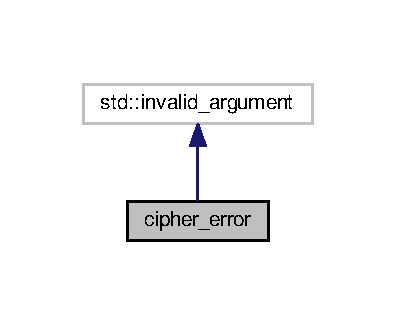
\includegraphics[width=190pt]{classcipher__error__inherit__graph}
\end{center}
\end{figure}


Граф связей класса cipher\+\_\+error\+:\nopagebreak
\begin{figure}[H]
\begin{center}
\leavevmode
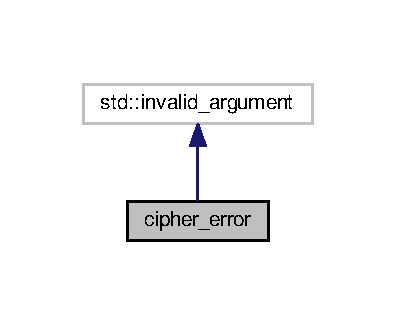
\includegraphics[width=190pt]{classcipher__error__coll__graph}
\end{center}
\end{figure}
\subsection*{Открытые члены}
\begin{DoxyCompactItemize}
\item 
{\bfseries cipher\+\_\+error} (const std\+::string \&what\+\_\+arg)\hypertarget{classcipher__error_aac662e216a84bfeb873303c7b88d029e}{}\label{classcipher__error_aac662e216a84bfeb873303c7b88d029e}

\item 
{\bfseries cipher\+\_\+error} (const char $\ast$what\+\_\+arg)\hypertarget{classcipher__error_a18cf27d9c2cd2538d3cb8f17e9a55f3e}{}\label{classcipher__error_a18cf27d9c2cd2538d3cb8f17e9a55f3e}

\end{DoxyCompactItemize}


Объявления и описания членов класса находятся в файле\+:\begin{DoxyCompactItemize}
\item 
\hyperlink{modAlphaCipher_8h}{mod\+Alpha\+Cipher.\+h}\end{DoxyCompactItemize}

\hypertarget{classmodAlphaCipher}{}\section{Класс mod\+Alpha\+Cipher}
\label{classmodAlphaCipher}\index{mod\+Alpha\+Cipher@{mod\+Alpha\+Cipher}}
\subsection*{Открытые члены}
\begin{DoxyCompactItemize}
\item 
\hyperlink{classmodAlphaCipher_a4f0a86c20f5d836f66cb1e640d875e6b}{mod\+Alpha\+Cipher} ()=delete\hypertarget{classmodAlphaCipher_a4f0a86c20f5d836f66cb1e640d875e6b}{}\label{classmodAlphaCipher_a4f0a86c20f5d836f66cb1e640d875e6b}

\begin{DoxyCompactList}\small\item\em Пустой конструктор для установки ключа.  Конструктор запрещён. \end{DoxyCompactList}\item 
\hyperlink{classmodAlphaCipher_a314fca132f4e74faca280b7c1fad7cb5}{mod\+Alpha\+Cipher} (const std\+::wstring \&skey)
\begin{DoxyCompactList}\small\item\em Конструктор для установки ключа. \end{DoxyCompactList}\item 
std\+::string \hyperlink{classmodAlphaCipher_a9b586f4aa0c7424294a4df87b474777d}{encrypt} (const std\+::wstring \&open\+\_\+text)
\begin{DoxyCompactList}\small\item\em Метод шифрования текста шифром Гронсфельда. \end{DoxyCompactList}\item 
std\+::string \hyperlink{classmodAlphaCipher_a8396673a3de84ddde862b11cd18de9b1}{decrypt} (const std\+::wstring \&cipher\+\_\+text)
\begin{DoxyCompactList}\small\item\em Метод шифрования текста шифром Гронсфельда. \end{DoxyCompactList}\end{DoxyCompactItemize}
\subsection*{Закрытые члены}
\begin{DoxyCompactItemize}
\item 
std\+::wstring \hyperlink{classmodAlphaCipher_a36544c603bcd87edcc33df0c8fa26c9f}{get\+Valid\+Key} (const std\+::wstring \&s)
\begin{DoxyCompactList}\small\item\em Валидация ключа. \end{DoxyCompactList}\item 
std\+::wstring \hyperlink{classmodAlphaCipher_a8e2be98736fee4107c92f5a8fcba4d1d}{get\+Valid\+Open\+Text} (const std\+::wstring \&s)
\begin{DoxyCompactList}\small\item\em Валидация открытого текста. \end{DoxyCompactList}\item 
std\+::wstring \hyperlink{classmodAlphaCipher_a67de093db93e0dab43381326d4da1835}{get\+Valid\+Cipher\+Text} (const std\+::wstring \&s)
\begin{DoxyCompactList}\small\item\em Валидация текста, требующего расшифровки. \end{DoxyCompactList}\item 
std\+::vector$<$ int $>$ \hyperlink{classmodAlphaCipher_a12ace58352c18bac7a7b61f312a4c8d6}{convert} (const std\+::wstring \&s)
\begin{DoxyCompactList}\small\item\em Преобразование \char`\"{}строка-\/вектор\char`\"{}. \end{DoxyCompactList}\item 
std\+::string \hyperlink{classmodAlphaCipher_afa3ddac1b01e7847238478963d667d4a}{convert} (const std\+::vector$<$ int $>$ \&v)
\begin{DoxyCompactList}\small\item\em Преобразование "вектор-\/строка. \end{DoxyCompactList}\end{DoxyCompactItemize}
\subsection*{Закрытые данные}
\begin{DoxyCompactItemize}
\item 
std\+::wstring \hyperlink{classmodAlphaCipher_ab7e0c7d3c87f4c8b7435d84f31c6cb62}{num\+Alpha}
\begin{DoxyCompactList}\small\item\em Русский алфавит по порядку. \end{DoxyCompactList}\item 
std\+::map$<$ wchar\+\_\+t, int $>$ \hyperlink{classmodAlphaCipher_ad896cbfa7d4c32d1c9627b0812b4a677}{alpha\+Num}\hypertarget{classmodAlphaCipher_ad896cbfa7d4c32d1c9627b0812b4a677}{}\label{classmodAlphaCipher_ad896cbfa7d4c32d1c9627b0812b4a677}

\begin{DoxyCompactList}\small\item\em Ассоциативный массив \char`\"{}номер по символу\char`\"{}. \end{DoxyCompactList}\item 
std\+::vector$<$ int $>$ \hyperlink{classmodAlphaCipher_aaddfb3bc0a3806b17e94c56fea5bad87}{key}\hypertarget{classmodAlphaCipher_aaddfb3bc0a3806b17e94c56fea5bad87}{}\label{classmodAlphaCipher_aaddfb3bc0a3806b17e94c56fea5bad87}

\begin{DoxyCompactList}\small\item\em Ключ \end{DoxyCompactList}\end{DoxyCompactItemize}


\subsection{Конструктор(ы)}
\index{mod\+Alpha\+Cipher@{mod\+Alpha\+Cipher}!mod\+Alpha\+Cipher@{mod\+Alpha\+Cipher}}
\index{mod\+Alpha\+Cipher@{mod\+Alpha\+Cipher}!mod\+Alpha\+Cipher@{mod\+Alpha\+Cipher}}
\subsubsection[{\texorpdfstring{mod\+Alpha\+Cipher(const std\+::wstring \&skey)}{modAlphaCipher(const std::wstring &skey)}}]{\setlength{\rightskip}{0pt plus 5cm}mod\+Alpha\+Cipher\+::mod\+Alpha\+Cipher (
\begin{DoxyParamCaption}
\item[{const std\+::wstring \&}]{skey}
\end{DoxyParamCaption}
)}\hypertarget{classmodAlphaCipher_a314fca132f4e74faca280b7c1fad7cb5}{}\label{classmodAlphaCipher_a314fca132f4e74faca280b7c1fad7cb5}


Конструктор для установки ключа. 

Устанавливает ключ, с помощью которого будет осуществляться шифрование и расшифрование. 
\begin{DoxyParams}[1]{Аргументы}
\mbox{\tt in}  & {\em skey} & Строка-\/ключ. Должна состоять из букв русского алфавита в верхнем регистре. Не должна быть пустой. Все символы в нижнем регистре будут автоматически преобразованы в верхний. \\
\hline
\end{DoxyParams}

\begin{DoxyExceptions}{Исключения}
{\em \hyperlink{classcipher__error}{cipher\+\_\+error},если} & строка пустая или содержит символы не русского алфавита или ключ вырожденный. \\
\hline
\end{DoxyExceptions}


\subsection{Методы}
\index{mod\+Alpha\+Cipher@{mod\+Alpha\+Cipher}!convert@{convert}}
\index{convert@{convert}!mod\+Alpha\+Cipher@{mod\+Alpha\+Cipher}}
\subsubsection[{\texorpdfstring{convert(const std\+::wstring \&s)}{convert(const std::wstring &s)}}]{\setlength{\rightskip}{0pt plus 5cm}std\+::vector$<$ int $>$ mod\+Alpha\+Cipher\+::convert (
\begin{DoxyParamCaption}
\item[{const std\+::wstring \&}]{s}
\end{DoxyParamCaption}
)\hspace{0.3cm}{\ttfamily [inline]}, {\ttfamily [private]}}\hypertarget{classmodAlphaCipher_a12ace58352c18bac7a7b61f312a4c8d6}{}\label{classmodAlphaCipher_a12ace58352c18bac7a7b61f312a4c8d6}


Преобразование \char`\"{}строка-\/вектор\char`\"{}. 


\begin{DoxyParams}[1]{Аргументы}
\mbox{\tt in}  & {\em s} & Строка, требущая конвертации в целочисленный вектор. \\
\hline
\end{DoxyParams}
\begin{DoxyReturn}{Возвращает}
Целочисленный вектор. 
\end{DoxyReturn}
\index{mod\+Alpha\+Cipher@{mod\+Alpha\+Cipher}!convert@{convert}}
\index{convert@{convert}!mod\+Alpha\+Cipher@{mod\+Alpha\+Cipher}}
\subsubsection[{\texorpdfstring{convert(const std\+::vector$<$ int $>$ \&v)}{convert(const std::vector< int > &v)}}]{\setlength{\rightskip}{0pt plus 5cm}std\+::string mod\+Alpha\+Cipher\+::convert (
\begin{DoxyParamCaption}
\item[{const std\+::vector$<$ int $>$ \&}]{v}
\end{DoxyParamCaption}
)\hspace{0.3cm}{\ttfamily [inline]}, {\ttfamily [private]}}\hypertarget{classmodAlphaCipher_afa3ddac1b01e7847238478963d667d4a}{}\label{classmodAlphaCipher_afa3ddac1b01e7847238478963d667d4a}


Преобразование "вектор-\/строка. 


\begin{DoxyParams}[1]{Аргументы}
\mbox{\tt in}  & {\em v} & Вектор, требующий преобразования в строку. \\
\hline
\end{DoxyParams}
\begin{DoxyReturn}{Возвращает}
Строка. 
\end{DoxyReturn}
\index{mod\+Alpha\+Cipher@{mod\+Alpha\+Cipher}!decrypt@{decrypt}}
\index{decrypt@{decrypt}!mod\+Alpha\+Cipher@{mod\+Alpha\+Cipher}}
\subsubsection[{\texorpdfstring{decrypt(const std\+::wstring \&cipher\+\_\+text)}{decrypt(const std::wstring &cipher_text)}}]{\setlength{\rightskip}{0pt plus 5cm}std\+::string mod\+Alpha\+Cipher\+::decrypt (
\begin{DoxyParamCaption}
\item[{const std\+::wstring \&}]{cipher\+\_\+text}
\end{DoxyParamCaption}
)}\hypertarget{classmodAlphaCipher_a8396673a3de84ddde862b11cd18de9b1}{}\label{classmodAlphaCipher_a8396673a3de84ddde862b11cd18de9b1}


Метод шифрования текста шифром Гронсфельда. 


\begin{DoxyParams}[1]{Аргументы}
\mbox{\tt in}  & {\em open\+\_\+text} & Текст, требующий расшифровки.\+Не должен быть пустой строкой. Должен содержать только символы русского алфавита в верхнем регистре. \\
\hline
\end{DoxyParams}

\begin{DoxyExceptions}{Исключения}
{\em \hyperlink{classcipher__error}{cipher\+\_\+error},если} & строка пустая, содержит символы не русского алфавита или символы в нижнем регистре. \\
\hline
\end{DoxyExceptions}
\index{mod\+Alpha\+Cipher@{mod\+Alpha\+Cipher}!encrypt@{encrypt}}
\index{encrypt@{encrypt}!mod\+Alpha\+Cipher@{mod\+Alpha\+Cipher}}
\subsubsection[{\texorpdfstring{encrypt(const std\+::wstring \&open\+\_\+text)}{encrypt(const std::wstring &open_text)}}]{\setlength{\rightskip}{0pt plus 5cm}std\+::string mod\+Alpha\+Cipher\+::encrypt (
\begin{DoxyParamCaption}
\item[{const std\+::wstring \&}]{open\+\_\+text}
\end{DoxyParamCaption}
)}\hypertarget{classmodAlphaCipher_a9b586f4aa0c7424294a4df87b474777d}{}\label{classmodAlphaCipher_a9b586f4aa0c7424294a4df87b474777d}


Метод шифрования текста шифром Гронсфельда. 


\begin{DoxyParams}[1]{Аргументы}
\mbox{\tt in}  & {\em open\+\_\+text} & Открытый текст.\+Не должен быть пустой строкой. Должен содержать только символы русского алфавита. Строчные символы автоматически преобразуются к прописным. Все не-\/буквы удаляются \\
\hline
\end{DoxyParams}

\begin{DoxyExceptions}{Исключения}
{\em \hyperlink{classcipher__error}{cipher\+\_\+error},если} & строка пустая. \\
\hline
\end{DoxyExceptions}
\index{mod\+Alpha\+Cipher@{mod\+Alpha\+Cipher}!get\+Valid\+Cipher\+Text@{get\+Valid\+Cipher\+Text}}
\index{get\+Valid\+Cipher\+Text@{get\+Valid\+Cipher\+Text}!mod\+Alpha\+Cipher@{mod\+Alpha\+Cipher}}
\subsubsection[{\texorpdfstring{get\+Valid\+Cipher\+Text(const std\+::wstring \&s)}{getValidCipherText(const std::wstring &s)}}]{\setlength{\rightskip}{0pt plus 5cm}std\+::wstring mod\+Alpha\+Cipher\+::get\+Valid\+Cipher\+Text (
\begin{DoxyParamCaption}
\item[{const std\+::wstring \&}]{s}
\end{DoxyParamCaption}
)\hspace{0.3cm}{\ttfamily [inline]}, {\ttfamily [private]}}\hypertarget{classmodAlphaCipher_a67de093db93e0dab43381326d4da1835}{}\label{classmodAlphaCipher_a67de093db93e0dab43381326d4da1835}


Валидация текста, требующего расшифровки. 


\begin{DoxyParams}[1]{Аргументы}
\mbox{\tt in}  & {\em s} & Текст, требующий расшифровки. \\
\hline
\end{DoxyParams}
\begin{DoxyReturn}{Возвращает}
Шифр-\/текст. 
\end{DoxyReturn}
\index{mod\+Alpha\+Cipher@{mod\+Alpha\+Cipher}!get\+Valid\+Key@{get\+Valid\+Key}}
\index{get\+Valid\+Key@{get\+Valid\+Key}!mod\+Alpha\+Cipher@{mod\+Alpha\+Cipher}}
\subsubsection[{\texorpdfstring{get\+Valid\+Key(const std\+::wstring \&s)}{getValidKey(const std::wstring &s)}}]{\setlength{\rightskip}{0pt plus 5cm}std\+::wstring mod\+Alpha\+Cipher\+::get\+Valid\+Key (
\begin{DoxyParamCaption}
\item[{const std\+::wstring \&}]{s}
\end{DoxyParamCaption}
)\hspace{0.3cm}{\ttfamily [inline]}, {\ttfamily [private]}}\hypertarget{classmodAlphaCipher_a36544c603bcd87edcc33df0c8fa26c9f}{}\label{classmodAlphaCipher_a36544c603bcd87edcc33df0c8fa26c9f}


Валидация ключа. 


\begin{DoxyParams}[1]{Аргументы}
\mbox{\tt in}  & {\em s} & Ключ \\
\hline
\end{DoxyParams}
\begin{DoxyReturn}{Возвращает}
Обработанный ключ. 
\end{DoxyReturn}
\index{mod\+Alpha\+Cipher@{mod\+Alpha\+Cipher}!get\+Valid\+Open\+Text@{get\+Valid\+Open\+Text}}
\index{get\+Valid\+Open\+Text@{get\+Valid\+Open\+Text}!mod\+Alpha\+Cipher@{mod\+Alpha\+Cipher}}
\subsubsection[{\texorpdfstring{get\+Valid\+Open\+Text(const std\+::wstring \&s)}{getValidOpenText(const std::wstring &s)}}]{\setlength{\rightskip}{0pt plus 5cm}std\+::wstring mod\+Alpha\+Cipher\+::get\+Valid\+Open\+Text (
\begin{DoxyParamCaption}
\item[{const std\+::wstring \&}]{s}
\end{DoxyParamCaption}
)\hspace{0.3cm}{\ttfamily [inline]}, {\ttfamily [private]}}\hypertarget{classmodAlphaCipher_a8e2be98736fee4107c92f5a8fcba4d1d}{}\label{classmodAlphaCipher_a8e2be98736fee4107c92f5a8fcba4d1d}


Валидация открытого текста. 


\begin{DoxyParams}[1]{Аргументы}
\mbox{\tt in}  & {\em s} & Открытый текст. \\
\hline
\end{DoxyParams}
\begin{DoxyReturn}{Возвращает}
Обработыннй открытый тест. 
\end{DoxyReturn}


\subsection{Данные класса}
\index{mod\+Alpha\+Cipher@{mod\+Alpha\+Cipher}!num\+Alpha@{num\+Alpha}}
\index{num\+Alpha@{num\+Alpha}!mod\+Alpha\+Cipher@{mod\+Alpha\+Cipher}}
\subsubsection[{\texorpdfstring{num\+Alpha}{numAlpha}}]{\setlength{\rightskip}{0pt plus 5cm}std\+::wstring mod\+Alpha\+Cipher\+::num\+Alpha\hspace{0.3cm}{\ttfamily [private]}}\hypertarget{classmodAlphaCipher_ab7e0c7d3c87f4c8b7435d84f31c6cb62}{}\label{classmodAlphaCipher_ab7e0c7d3c87f4c8b7435d84f31c6cb62}
{\bfseries Инициализатор}
\begin{DoxyCode}
=
        L\textcolor{stringliteral}{"АБВГДЕЁЖЗИЙКЛМНОПРСТУФХЦЧШЩЪЫЬЭЮЯ"}
\end{DoxyCode}


Русский алфавит по порядку. 



Объявления и описания членов классов находятся в файлах\+:\begin{DoxyCompactItemize}
\item 
\hyperlink{modAlphaCipher_8h}{mod\+Alpha\+Cipher.\+h}\item 
mod\+Alpha\+Cipher.\+cpp\end{DoxyCompactItemize}

\chapter{Файлы}
\hypertarget{modAlphaCipher_8h}{}\section{Файл mod\+Alpha\+Cipher.\+h}
\label{modAlphaCipher_8h}\index{mod\+Alpha\+Cipher.\+h@{mod\+Alpha\+Cipher.\+h}}


Заголовочный файл для модуля \hyperlink{classmodAlphaCipher}{mod\+Alpha\+Cipher}.  


{\ttfamily \#include $<$vector$>$}\\*
{\ttfamily \#include $<$codecvt$>$}\\*
{\ttfamily \#include $<$string$>$}\\*
{\ttfamily \#include $<$map$>$}\\*
Граф включаемых заголовочных файлов для mod\+Alpha\+Cipher.\+h\+:\nopagebreak
\begin{figure}[H]
\begin{center}
\leavevmode
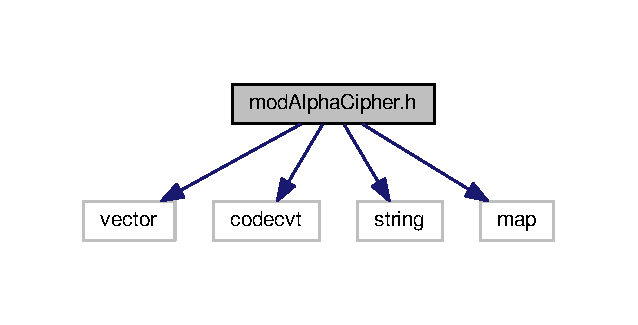
\includegraphics[width=306pt]{modAlphaCipher_8h__incl}
\end{center}
\end{figure}
\subsection*{Классы}
\begin{DoxyCompactItemize}
\item 
class \hyperlink{classmodAlphaCipher}{mod\+Alpha\+Cipher}
\item 
class \hyperlink{classcipher__error}{cipher\+\_\+error}
\end{DoxyCompactItemize}


\subsection{Подробное описание}
Заголовочный файл для модуля \hyperlink{classmodAlphaCipher}{mod\+Alpha\+Cipher}. 

\begin{DoxyAuthor}{Автор}
Асаян А.\+В. 
\end{DoxyAuthor}
\begin{DoxyVersion}{Версия}
1.\+0 
\end{DoxyVersion}
\begin{DoxyDate}{Дата}
28.\+05.\+2019 
\end{DoxyDate}
\begin{DoxyCopyright}{Авторство}
ИБСТ ПГУ 
\end{DoxyCopyright}
\begin{DoxyWarning}{Предупреждения}
Работа студента. 
\end{DoxyWarning}

%--- End generated contents ---

% Index
\backmatter
\newpage
\phantomsection
\clearemptydoublepage
\addcontentsline{toc}{chapter}{Алфавитный указатель}
\printindex

\end{document}
